\section{HIP (Points 3/3)}
Successfully Implemented the classical CG Algorithm in HIP. Whereby "implmenting" I mean replacing \fun{CUDA} commands to \fun{HIP} commands.
A bit trickier where the Kernel calls, But eventually made it run and it still converges and yields corrects results (Relative residual error smaller than 1e-6).

\begin{figure}[h]
    \begin{center}
        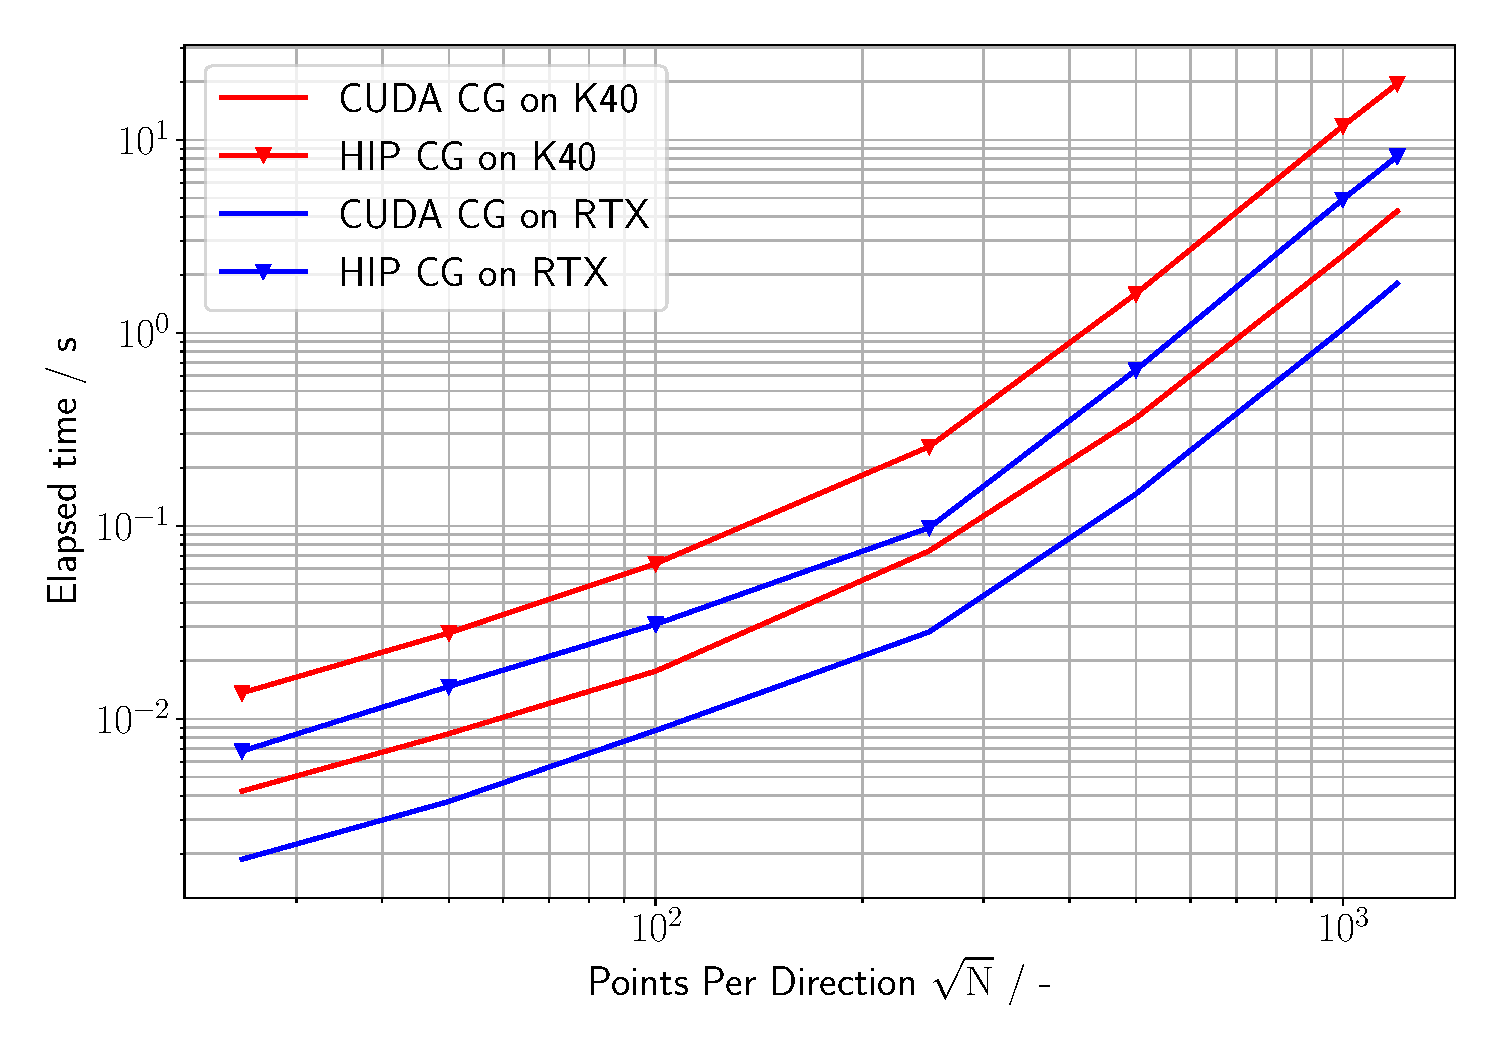
\includegraphics[width = \linewidth]{figures/task_9_2_plot.pdf}
        \caption{Comparison Conjugate Gradient Algorithm with \fun{CUDA} and \fun{HIP}}
        \end{center}
\end{figure}

The HIP Implementation is slower for both GPU's!

\section{BONUS: Relaxed Christmas Break (0/1 Point)}
I had a very relaxed christmas break, therefore You could grant me the Bonus point!
Jokes aside, I hope You had a very relaxed Christmas break! :-) Kind regards.